%%%%%%%%%%%%%%%%%%%%%%%%%%%%%%%%%%%%%%%%%%%%%%%%%%%%%%%%%%%%%%%%%%%%%%%%
% Copyright (c) 2022 Antonio Coín
%
% This work is licensed under a
% Creative Commons Attribution-ShareAlike 4.0 International License.
%
% You should have received a copy of the license along with this
% work. If not, see <http://creativecommons.org/licenses/by-sa/4.0/>.
%%%%%%%%%%%%%%%%%%%%%%%%%%%%%%%%%%%%%%%%%%%%%%%%%%%%%%%%%%%%%%%%%%%%%%%%

\let\epsilon\varepsilon

%%%%%%%%%%%%%%%%%%%%%%%%%%%%%%%%%%%%%%%%%%%%%%%%%%%%%%%%%%%%%%%%%%%%%%%%
\chapter{Experiments}\label{ch:experiments}
%%%%%%%%%%%%%%%%%%%%%%%%%%%%%%%%%%%%%%%%%%%%%%%%%%%%%%%%%%%%%%%%%%%%%%%%

In this chapter we present the results of the experiments carried out to test the performance of our models in different scenarios. The structure of the code and other minor computational details are discussed in Appendix~\ref{ch:code}.

\subsection*{Experimental setting}

First and foremost, we consider \(T=\{\text{mean, median, mode}\}\) for the summarize-then-predict approach to prediction. In this way in linear regression we have 4 prediction methods (one for each statistic and one for the predict-then-summarize approach, which will we call ``\textit{posterior\_mean}'' for short) and 3 variable selection methods (one for each statistic), while in logistic regression there are similarly 5 prediction methods and 3 variable selection procedures. In each case, after variable selection is performed, we use a penalized multiple linear/logistic regression method to generate the corresponding predictions. All in all, we are looking at 7 (8 in the case of logistic regression) prediction methods, and although all of them are derived from a single MCMC run, we will treat them as separate for the purposes of the experimentation. In what follows we relax the notation and use the expressions ``model'', ``prediction method'' and ``algorithm'' almost interchangeably when referring to these 7 (or 8) cases.

We consider \(n=150\) training samples and \(n'=100\) testing samples on an equispaced grid of \(N=100\) points on \([0, 1]\) for the simulated data sets, and we do a 66\%/33\% train/test split on the real data sets. We then perform \(5\)-fold cross validation (CV) on the training set to select the best values of \(p\) and \(\eta\) for each model, and after refitting the best model in each case on the whole training set, we evaluate it and measure the predictive performance on the test set. We look for \(p\) in the set \(\{1,2,\dots,10\}\), while the possible values of \(\eta\) are \(\{10^{-4}, 10^{-3}, \dots, 10^2\}\).

Because of execution time constraints, the hyperparameters of the MCMC method are not part of the CV process, and are selected manually based on an initial set of experiments, as well as recommendations from the original article. We use 64 chains and run them for 900 iterations in total, discarding the first 500 iterations as burn-in. Moreover, we use a weighted mixture of walk and stretch moves in the \textit{emcee} sampler to advance the chains at each iteration, selecting the stretch move (the default) with probability \(0.7\), or the walk move with probability \(0.3\).

Lastly, since the use of MCMC algorithms introduces a source of stochasticity in the prediction procedure, we independently repeat the whole process 10 times (each with a different train/test configuration), and average the results across these executions. The metrics used to evaluate the performance of the models are the RMSE for linear regression and the accuracy for logistic regression. Recall that
\[
\operatorname{RMSE}(\{\hat y_i\}) = \sqrt{\frac{1}{n'}\sum_{i=1}^{n'} (y_i - \hat y_i)^2}
\]
and
\[
\operatorname{Accuracy}(\{\hat y_i\}) = \frac{1}{n'} \sum_{i=1}^{n'} \I(y_i = \hat y_i).
\]

\subsection*{Data sets}

We consider a set of functional regressors common to linear and logistic regression problems. They are 4 Gaussian processes (GP's), each with a different kernel function:
\begin{enumerate}
  \item BM.\hspace{0.3em} A Brownian motion \(K_1(t,s)=\min\{t,s\}\).
  \item fBM.\hspace{0.3em} A fractional Brownian motion \(K_2(t,s)=1/2(s^{2H} + t^{2H} - |t-s|^{2H})\), with Hurst parameter \(H=0.8\).
  \item O-U.\hspace{0.3em} An Ornstein-Uhlenbeck process \(K_3(t,s)=e^{-|t-s|}\).
  \item Gaussian.\hspace{0.3em} A Gaussian kernel \(K_4(t,s)=e^{-(t-s)^2/2\nu^2}\), with \(\nu=0.2\).
\end{enumerate}
Also, when applicable, we fix a variance \(\sigma^2=0.5\) for the error terms \(\epsilon\).

\paragraph{Linear regression data sets.} We consider three different types of data sets, all with a common value of \(\alpha_0=5\).
\begin{itemize}
  \item A RKHS model where the response is generated as \(Y= 0.5 -5X(0.1) + X(0.4) + 10X(0.8) + \epsilon\), for each of the four GP's mentioned above.
  \item A \(L^2\)-model with underlying coefficient function \(\beta(t)=\log(1+4t)\), again for the same four GP's.
  \item A model based on non-GP regressors. Specifically, we use a geometric Brownian motion (GBM) defined as \(X(t)=e^{BM(t)}\), where \(BM(t)\) is a standard Brownian motion. In this case, we consider two data sets, one with a RKHS response and one with a \(L^2\) response, with the same parameters as above.
\end{itemize}
As for the real data sets, we use the (twice-differentiated) Tecator data set introduced in Chapter~\ref{ch:introduction} to predict fat content of 193 meat samples, as well as what we call the Moisture \citep{kalivas1997two} and Sugar \citep{bro1999exploratory} data sets. The first consists of near-infrared spectra of 100 wheat samples and the objective is to predict the samples' moisture content, whereas the second contains 268 samples of sugar fluorescence data in order to predict ash content. The three data sets are measured on a grid of 100, 101 and 115 equispaced points in \([0, 1]\), respectively.

\paragraph{Logistic regression data sets.} Again we consider three different types of data sets,  with a common value of \(\alpha_0=-0.5\). In this case we randomly permute 10\% of the labels to introduce some noise in the simulations.
\begin{itemize}
  \item Four logistic RKHS models with the same functional parameter as in the linear regression case (one for each GP). Specifically,
  \[
  \P(Y=1\mid X) = \frac{1}{1 + e^{0.5 +5X(0.1) - X(0.4) - 10X(0.8)}}.
  \]
  \item Four logistic \(L^2\)-models with the same coefficient function as in the linear regression case.
  \item A ``mixture'' model based on non-GP regressors, in which we mix regressors from two different GP's (with equal probability \(p=1/2\)) and label them according to their origin. Firstly, we consider a homoscedastic case to distinguish between a standard Brownian motion and a Brownian motion with a mean function that is zero until \(t=0.5\), and then becomes \(m(t)=0.75t\). Secondly, we consider a heteroscedastic case to distinguish between a standard Brownian motion and a Brownian motion with variance \(2\), that is, with kernel \(K(t,s)=2\min\{t,s\}\).
\end{itemize}
In this case there are again three real data sets. The first one is a subset of the Medflies data set \citep{carey1998relationship}, consisting on samples of the number of eggs laid daily by 534 flies over 30 days, trying to predict if their longevity is high or low. The second one is the Berkeley Growth Study data set \citep{tuddenham1954physical}, which records the height of 54 girls and 39 boys over 31 different points in their lives. Finally, we have selected a subset of the Phoneme data set \citep{hastie1995penalized}, based on 200 digitized speech frames over 128 equispaced points to predict the phonemes ``aa'' and ``ao''.

\subsection*{Comparison algorithms}

We have included a fairly comprehensive suite of comparison algorithms, chosen among the most common methods used in machine learning and FDA. There are finite-dimensional models that work on the discretized data, variable selection/dimension reduction procedures and purely functional methods.

\paragraph{Linear regression comparison algorithms.} We consider the following methods.
\begin{itemize}
  \item Manual.\hspace{.3em} Dummy variable selection method with a pre-specified number of components (equispaced on \([0, 1]\)).
  \item Lasso.\hspace{.3em} Linear least squares with \(l^1\) regularization.
  \item Ridge.\hspace{.3em} Linear least squares with \(l^2\) regularization.
  \item PLS.\hspace{.3em} Partial least squares for dimension reduction.
  \item PCA.\hspace{.3em} Principal component analysis for dimension reduction.
  \item PLS1.\hspace{.3em} Partial least squares regression \citep[e.g.][]{wegelin2000survey}.
  \item APLS.\hspace{.3em} Functional partial least squares regression proposed by \citet{delaigle2012methodology}.
  \item RMH.\hspace{.3em} Recursive maxima hunting variable selection method proposed by \citet{torrecilla2016feature}.
  \item FLin.\hspace{.3em} Functional \(L^2\) linear regression model with fixed basis expansion.
  \item FPLS1.\hspace{.3em} Functional PLS regression through basis expansion, implemented as in \citet{aguilera2010using}.
  \item FPCA.\hspace{.3em} Functional principal component analysis.
\end{itemize}

\paragraph{Logistic regression comparison algorithms.} All the variable selection and dimension reduction algorithms from above are also considered in this case.
\begin{itemize}
  \item Log.\hspace{.3em} Standard multiple logistic regression with \(l^2\) regularization.
  \item LDA.\hspace{.3em} Linear discriminant analysis.
  \item QDA.\hspace{.3em} Quadratic discriminant analysis.
  \item RKVS.\hspace{.3em} RKHS-based variable selection method proposed in \citet{berrendero2018use}.
  \item APLS.\hspace{.3em} Functional PLS used as a dimension reduction method, as proposed in \citet{delaigle2012achieving} in combination with the nearest centroid algorithm.
  \item FLog.\hspace{.3em} Functional RKHS-based logistic regression algorithm proposed in \citet{berrendero2018functional}.
  \item FLDA.\hspace{.3em} Implementation of the so-called functional linear discriminant analysis in \citet{preda2007pls}.
  \item MDC.\hspace{.3em} Maximum depth classifier \citep[e.g.][]{ghosh2005maximum}.
  \item FKNN.\hspace{.3em} Functional K-nearest neighbors classifier with the \(L^2\)-distance.
  \item FNC.\hspace{.3em} Functional nearest centroid classifier with the \(L^2\)-distance.
\end{itemize}

The main parameters of all these algorithms are selected by cross-validation, using the same 5 folds as our proposed models so that the comparisons are fair. In particular, the regularization parameter is searched among 20 values in the logarithmic space \([10^{-4}, 10^4]\), the number of manually selected variables is one of \(\{5, 10, 15, 20, 25, 50\}\), the number of components for dimension reduction and variable selection techniques is in the set \(\{2, 3, 4, 5, 7, 10, 15, 20\}\), the number of basis elements for quadratic spline bases is in \(\{8,10,12,14,16\}\), the number of basis elements for Fourier bases is one of \(\{3,5,7,9,11\}\), and the number of neighbors in the KNN classifier is in \(\{3,5,7,9,11\}\).

Most algorithms have been taken from the libraries \textit{scikit-learn}\footnote{\url{https://scikit-learn.org/stable/}} and \textit{scikit-fda}\footnote{\url{https://fda.readthedocs.io/en/latest/}}, the first oriented to machine learning in general and the second to functional data analysis in particular. However, some methods were not found in these packages and had to be implemented from scratch. This is the case of the FLDA, FPLS and APLS methods, which we coded following the corresponding articles.

\subsection*{Results display}

We have adopted a visual approach to presenting the experimentation results, using colored graphs to help visualize them. We felt that this was a better way of summarizing a large empirical study such as the one we have carried out. Alternatively, tables representing these results can be consulted in Appendix~\ref{ch:tables}.

We show the mean and standard deviation of the score obtained in each case across the 10 random runs, depicting our models in orange and the comparison algorithms in blue. We also show the global mean of all the comparison algorithms with a dashed vertical line, and we exclude extreme negative results from this mean to avoid distortion. Moreover, we separate complete prediction algorithms from two-stage methods, the latter being the ones that perform variable selection or dimension reduction prior to a multiple linear/logistic regression method.

We do not expect our models to defeat all the comparison algorithms in all cases (and indeed they do not), but we intend to show that they are competitive methods that on average match or improve the performance of other usual alternatives. After all, \textit{there is no such thing as a free lunch}\footnote{The phrase alludes to the No Free Lunch theorem, which loosely speaking asserts that all machine learning methods are equivalent when their performance is averaged across all possible problems. However, the practical implications of this statement are questionable \citep[see e.g.][]{giraud2005toward}.}!

\section{Functional linear regression}\label{sec:experiments-linear}

\subsection*{Simulated data sets}

In Figure~\ref{fig:reg_emcee_rkhs} we see the results for the four GP regressors considered in the RKHS case. This is the most favorable case for us, as the underlying model coincides with our assumed model. Indeed, we can see that in most cases our algorithms are the ones with lower RMSE, save for a few exceptions, notably with the Gaussian kernel. A subsequent analysis showed that this particular data set is especially sensitive to the value of the hyperparameter \(\eta\) in our prior distribution, so a more tailored approach would be needed to obtain better results.

\begin{figure}[ht!]
  \centering
  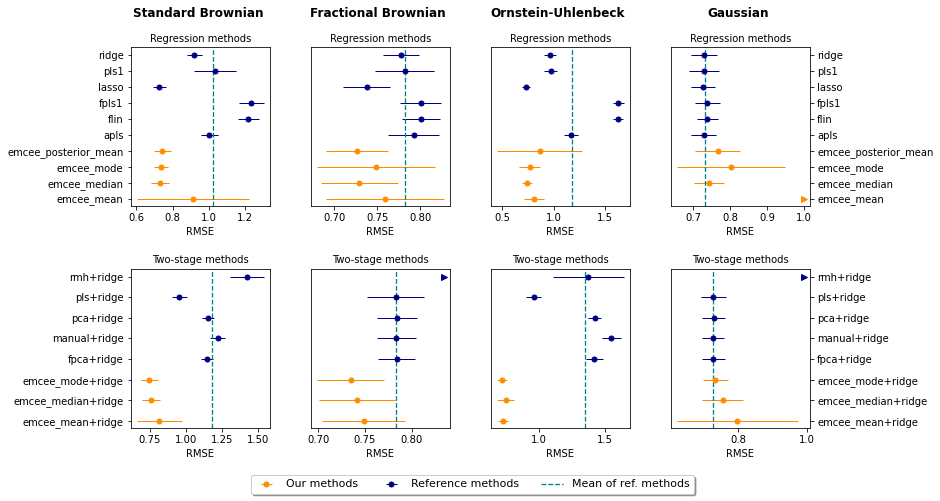
\includegraphics[width=\textwidth]{reg_emcee_rkhs}
  \caption{RMSE of predictors for simulated GP data that obeys an underlying RKHS model (lower is better).}\label{fig:reg_emcee_rkhs}
\end{figure}

In Figure~\ref{fig:reg_emcee_l2} we see the results for the case with an underlying \(L^2\)-model, which would be our most direct competitor. In this case the outcome is satisfactory, since for the most part our models are on a par with the rest, even beating other methods that were designed with the \(L^2\)-model in mind. Moreover, whenever one of our models has a higher RMSE, the difference is pretty small in comparison.
\begin{figure}[ht!]
  \centering
  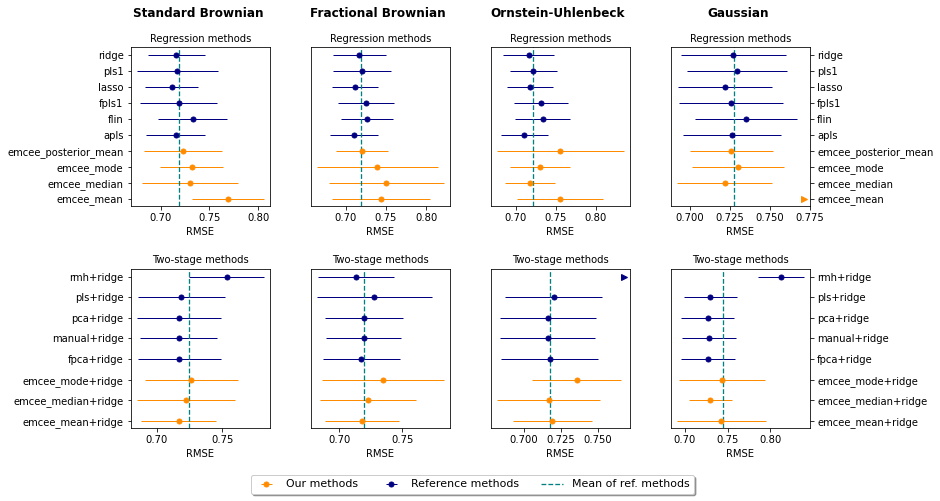
\includegraphics[width=\textwidth]{reg_emcee_l2}
  \caption{RMSE of predictors for simulated GP data that obeys an underlying \(L^2\) model (lower is better).}\label{fig:reg_emcee_l2}
\end{figure}

Note that some of our Bayesian models have a higher standard deviation, partly because there is an intrinsic randomness in the methods (apart from the train/test splits), and it can be the cause of the occasional worse performance. In relation to this, we observe that the methods that use the mean as a summary statistic tend to perform much worse. This is because the mean is very sensitive to outliers, so if at some point there is a chain that randomly deviates from the rest, the mean of the posterior distribution will be greatly impacted. In particular, very high values of the parameter \(\sigma^2\) were reported sometimes, producing misleading results when averaged with the rest of the values.

Lastly, the results for the non-GP case can be seen in Figure~\ref{fig:reg_emcee_nongp}, in which the regressors are realizations of a GBM. In this case we still get better results under the RKHS model, while the results under the \(L^2\)-model are slightly worse. However, as before, the difference is small (except for the \textit{emcee\_mean} methods).

\begin{figure}[ht!]
  \centering
  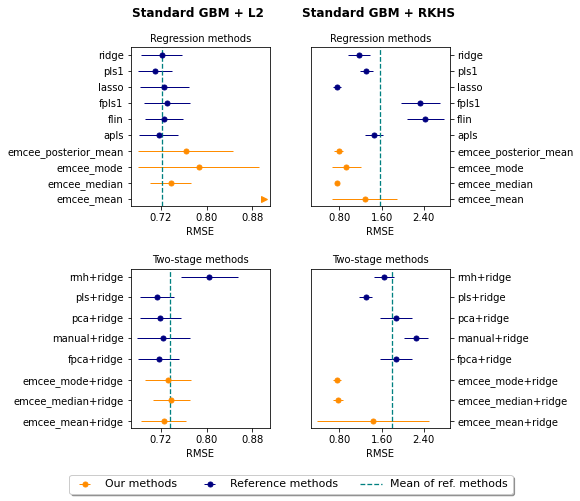
\includegraphics[width=.7\textwidth]{reg_emcee_nongp}
  \caption{RMSE of predictors for simulated data with GBM regressors (lower is better).}\label{fig:reg_emcee_nongp}
\end{figure}

\subsection*{Real data}

Figure~\ref{fig:reg_emcee_real} shows the results for the real data sets. In these data sets there is a substantial difference in performance between some of our methods and the reference algorithms. However, the predict-then-summarize approach (represented as \textit{posterior\_mean}) seems to work quite well, always scoring near the mean RMSE of all the comparison algorithms. Moreover, our two-stage methods seem to perform better than our other methods in these cases, scoring again very close to the mean of the reference methods.

We have to bear in mind that real data is more complex and noisy than simulated data, and it is possible that after a suitable pre-preprocessing we could obtain better results with our methods. However, our goal was to perform a general comparison without exploring too much to the specifics of any particular data set.

\begin{figure}[ht!]
  \centering
  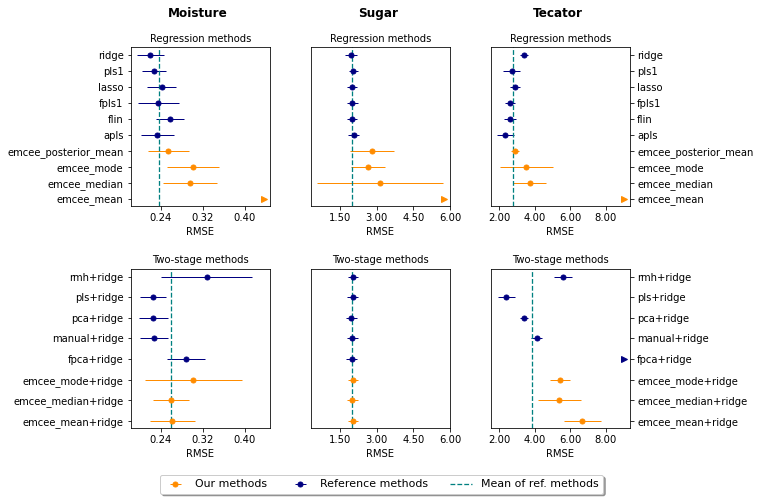
\includegraphics[width=.85\textwidth]{reg_emcee_real}
  \caption{RMSE of predictors for real data sets (lower is better).}\label{fig:reg_emcee_real}
\end{figure}

\section{Functional logistic regression}\label{sec:experiments-logistic}

\subsection*{Simulated data sets}

In Figure~\ref{fig:clf_emcee_rkhs} we see the results for the GP regressors in the logistic RKHS case. Our models perform fairly well in this advantageous case, although the two-stage methods fare somewhat poorly in these data sets. However, in most cases the differences observed account for only one or two misclassified samples.

\begin{figure}[ht!]
  \centering
  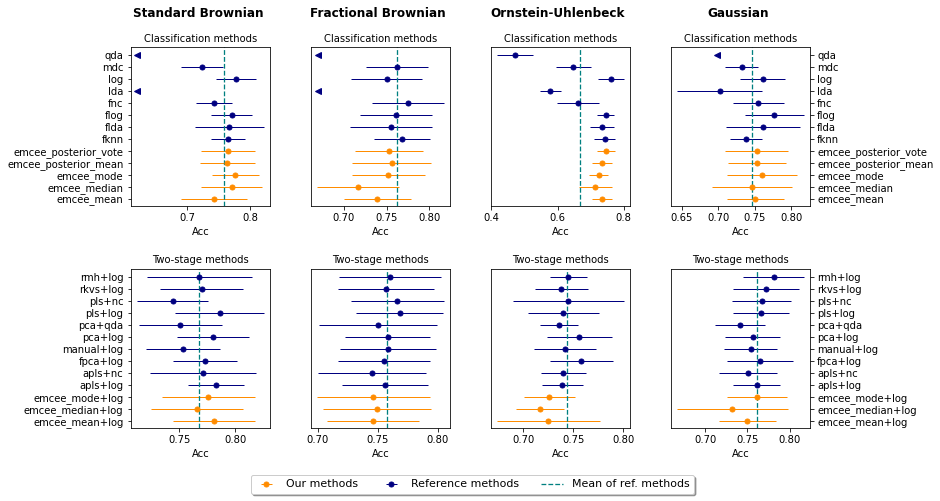
\includegraphics[width=\textwidth]{clf_emcee_rkhs}
  \caption{Accuracy of classifiers for simulated GP data that obeys an underlying logistic RKHS model (higher is better).}\label{fig:clf_emcee_rkhs}
\end{figure}

Continuing with Figure~\ref{fig:clf_emcee_l2}, we see that in the \(L^2\) case the results are again promising, since our models score consistently on or above the mean of the reference models, and in many cases surpassing most of them. The predict-then-summarize approaches (\textit{emcee\_posterior\_mean} and \textit{emcee\_posterior\_vote}) are particularly good in this case, and in general have low standard errors. Moreover, the overall accuracy of all methods is low (below 60\%), so this is indeed a difficult problem in which even small increases in accuracy are relevant.

\begin{figure}[ht!]
  \centering
  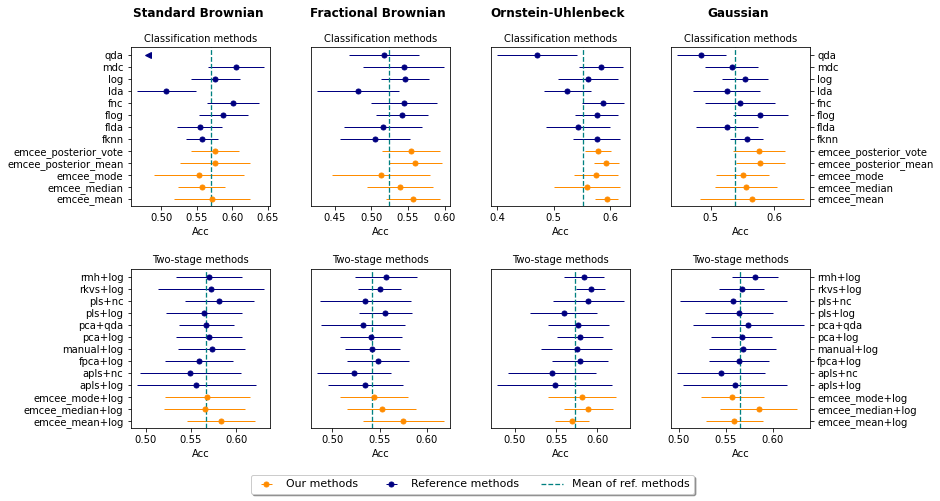
\includegraphics[width=\textwidth]{clf_emcee_l2}
  \caption{Accuracy of classifiers for simulated GP data that obeys an underlying logistic \(L^2\)-model (higher is better).}\label{fig:clf_emcee_l2}
\end{figure}

Finally, Figure~\ref{fig:clf_emcee_nongp} shows that our classifiers perform better than most comparison algorithms when separating two homoscedastic processes, but they struggle in the heteroscedastic case. Incidentally, this heteroscedastic case of two zero-mean Brownian motions has a special interest, since it can be shown that the Bayes error is zero in the limit of dense monitoring (i.e. with an arbitrarily fine measurement grid), a manifestation of the ``near-perfect'' classification phenomenon analyzed for example in \citet{torrecilla2020optimal}. Our results are in line with the empirical studies of said article, where the authors conclude that even though the asymptotic theoretical error is zero, most methods are suboptimal in practice (possibly due to the high collinearity of the data), with the notable exception of PCA+QDA.

\begin{figure}[ht!]
  \centering
  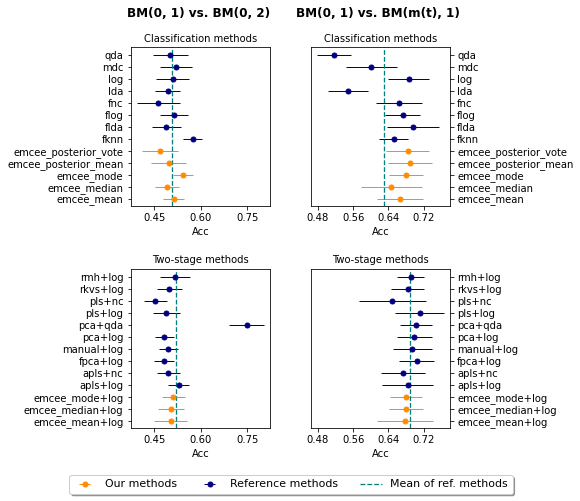
\includegraphics[width=.7\textwidth]{clf_emcee_nongp}
  \caption{Accuracy of classifiers for simulated data coming from two different GP's, labeled according to their origin (higher is better).}\label{fig:clf_emcee_nongp}
\end{figure}

\subsection*{Real data}

As for the real data sets, in Figure~\ref{fig:clf_emcee_real} we see positive results in general, obtaining in most cases accuracies well above the mean of the reference models, and sometimes above most of them. In particular, the predict-then-summarize tend to have a good performance and achieve a lower standard error across executions, which is a trend that we also saw in the simulated data sets. However, our variable selection methods seem to be a bit worse in this case. Again, the models that use \textit{emcee\_mean} are the exception, and in all these data sets they perform steadily worse than the rest of our Bayesian models.

\begin{figure}[ht!]
  \centering
  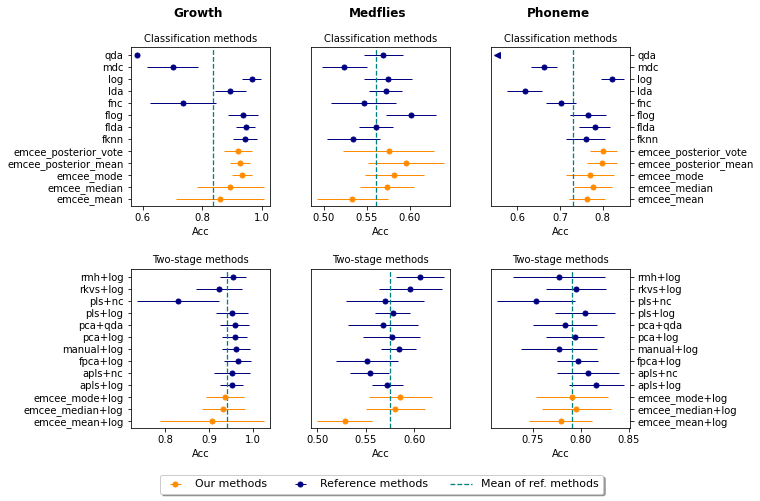
\includegraphics[width=.85\textwidth]{clf_emcee_real}
  \caption{Accuracy of classifiers for real data sets (higher is better).}\label{fig:clf_emcee_real}
\end{figure}


\section{Additional experiments}

In this section we present some experiments that are not directly related to measuring the prediction performance of our models relative to other methods.

\subsection*{Model misspecification}

One requirement that our model should satisfy is that it should be able to recover the true parameter function when the underlying model is a RKHS model. This is generally the case when the value of \(p\) in our model and the true value of \(p\) coincide, but what happens when we change the value of \(p\) in the model?

Take for example a data set generated according to the formula \(Y=-5X(0.1) + 10X(0.8) + \epsilon\), with \(\epsilon\sim \mathcal N(0, 0.5)\). Figure~\ref{fig:beta_trace_3} shows the resulting posterior distribution of the parameters \(b=(\beta_1, \beta_2, \beta_3)\) and \(\tau=(\tau_1, \tau_2, \tau_3)\) for a model with 3 components. As we can see, one of the coefficients has gone to zero to account for the overspecification of the model, while the other two have stabilized very close to the true parameters. The same goes for the time instants, except that in this case there is no default value to represent that a component is unused, so the time corresponding to the null coefficient oscillates back and forth. The estimated function (based for example in the mode of the posterior distributions) will not be perfect, essentially because of the noise in the response. But it should be close to the true parameter function \(\alpha(t)=-5K(t, 0.1) + 10K(t, 0.8)\), providing a good predictive performance.

\begin{figure}[ht!]
  \centering
  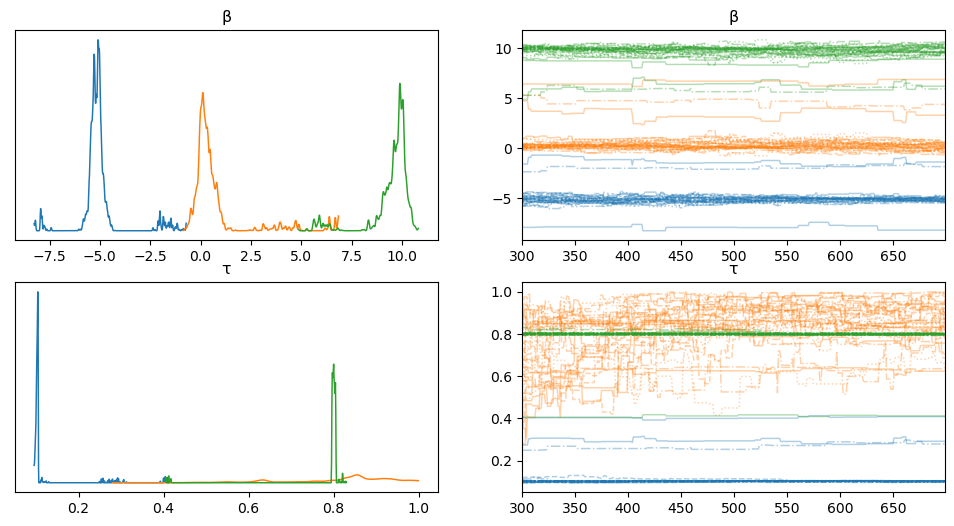
\includegraphics[width=.8\textwidth]{beta_trace_3}
  \caption{Estimated posterior distribution for \(\beta\) and \(\tau\) in a linear model with \(p=3\) (left) and the corresponding trace evolution for 700 iterations in the MCMC sampler (right).}\label{fig:beta_trace_3}
\end{figure}

In contrast, if we consider now a model with \(p=4\) with the same data, we might obtain posterior distributions like the ones in Figure~\ref{fig:beta_trace_4}. In this situation two coefficients should go to zero, but that is no longer the case. For example, while the green component has a high density around 0, it also has a considerable mass around 10, effectively ``competing'' with the red component. This is a manifestation of the label switching issue, caused in this case by an excessive number of degrees of freedom in the model.

\begin{figure}[ht!]
  \centering
  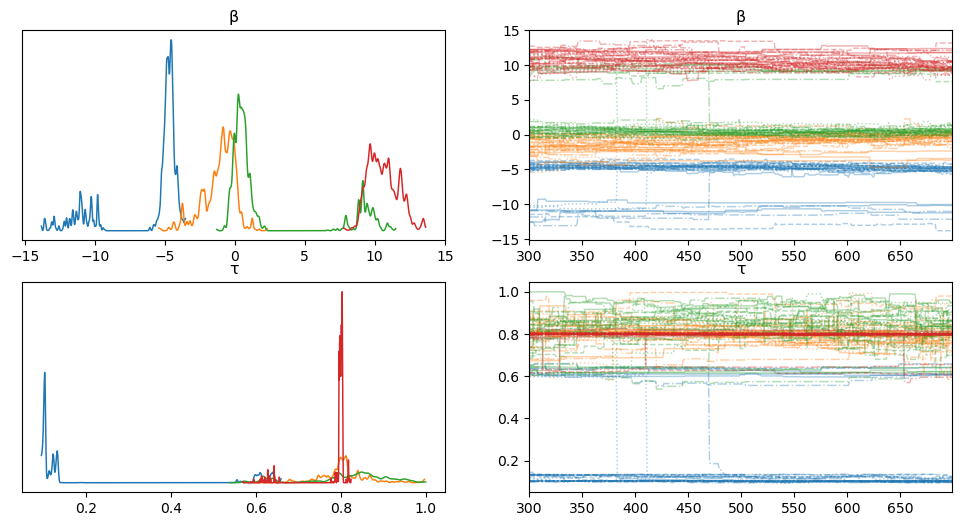
\includegraphics[width=.8\textwidth]{beta_trace_4}
  \caption{Estimated posterior distribution for \(\beta\) and \(\tau\) in a linear model with \(p=4\) (left) and the corresponding trace evolution for 700 iterations in the MCMC sampler (right).}\label{fig:beta_trace_4}
\end{figure}

There is still another possible situation, one in which there is no label switching but the estimated function has four non-negligible components. This can happen because the different components exploit the additional freedom and ``work together'', so to speak. In this way we might obtain an estimate that does not resemble the true coefficient function, but that has a very low prediction error. However, this could also work to our detriment and cause the estimated function to be worse prediction-wise than simpler alternatives. This phenomenon is expected to strengthen as the difference between the true and assumed value of \(p\) grows larger.

\subsection*{Dependence on \(p\)}

Another thing we wanted to look at was the dependence of the final prediction result on the chosen value of \(p\), especially when there is no concept of ``components'' in the underlying model. We can take for example the homoscedastic mixture data set in the logistic regression problem, and fix the parameter \(\eta=0.01\). Then the corresponding mean accuracies (in 10 repetitions) for RKHS models with \(p=1,2,\dots 10\) components are shown in Figure~\ref{fig:dependence_acc_p}, along with their standard errors (which are arguably not very informative).

\begin{figure}[ht!]
  \centering
  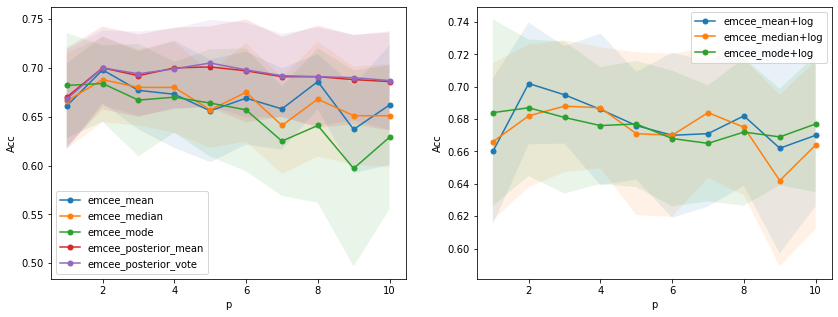
\includegraphics[width=0.9\textwidth]{mixture_dependence_acc_p}
  \caption{Mean accuracy in 10 repetitions for our logistic RKHS methods as a function of \(p\), using \(\eta=0.01\) and the homoscedastic mixture data set. The corresponding standard errors are shown in faded colors.}\label{fig:dependence_acc_p}
\end{figure}

It would appear that in the methods that use the whole posterior distribution are more stable and somewhat independent of the value of \(p>1\). The other methods show a slight downward trend as \(p\) increases (although not so much in the variable selection methods), and in general their best results are obtained at \(p=2\) and \(p=8\). We expect that this effect or some small variation of it will remain valid in other situations; however, a profound study of this would be the subject of a different experiment altogether.

\subsection*{Execution times}

We summarize below the mean execution time for each independent run of our CV experiment, grouping the simulated data sets by the underlying data generation strategy (since the results within these groups were very similar).

\begin{table}[ht!]
  \centering
  \begin{tabular}{lcccccc}
\toprule
  &            RKHS &           \(L^2\) &           GBM &        Tecator & Moisture & Sugar \\
\midrule
Linear regression & 260 & 245 & 264 & 230 & 264 & 285\\
\bottomrule

  &            RKHS &           \(L^2\) &           Mixture &        Medflies & Growth & Phoneme \\
\toprule
Logistic regression & 277 & 263 & 246 & 250 & 218 & 277\\
\bottomrule
\end{tabular}
  \caption{Mean execution times (in minutes) for the independent runs of the CV experiments in Sections~\ref{sec:experiments-linear} and~\ref{sec:experiments-logistic}, grouped when possible by the underlying data generation strategy.}
\end{table}

The reference algorithms used were all fast methods that can complete their whole CV loop in just a few seconds, so any comparison with them in this regard is uninteresting. However, this outcome was to be expected, since in general the MCMC methods are known to have a high computational cost in exchange for the simplicity in modeling they provide. An individual MCMC run is not that expensive time-wise, but even for a modest 5-fold cross-validation loop the effects add up quickly to a considerable amount of time. In Figure~\ref{fig:dependence_time_n_train} we show the evolution of the execution time versus the number of training samples in a generic case, which not surprisingly has a more or less linear behavior.

\begin{figure}[ht!]
  \centering
  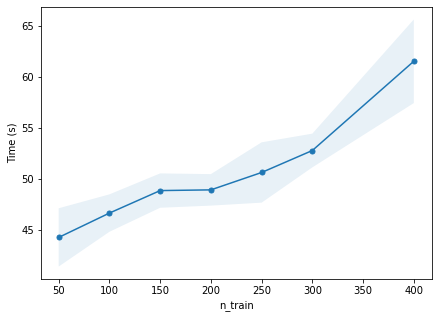
\includegraphics[width=0.6\textwidth]{l2_dependence_time_n_train}
  \caption{Mean training times of a logistic RKHS model, averaged across 10 independent runs, as a function of the number of training samples. The values are surrounded by the corresponding standard deviations. }\label{fig:dependence_time_n_train}
\end{figure}

\subsection*{Non-reported experiments}

Apart from all the experiments described above, we performed several tests with different configurations and alternatives. Although these trials did not produce better results in general, we mention some of them here to show how the model could be easily extended. In fact, many of these modifications, if not all, are still available in the provided code and can be enabled through specific parameters.

The first thing we tried was to make the parameter \(p\) part of the Bayesian model, imposing a categorical prior distribution on it. As explained in Chapter~\ref{ch:model-choice}, this approach led to many complications and generally poor results. However, the idea of letting the model select how many components it should have based on the data is an interesting one, and in some situations this could greatly improve the results of variable selection procedures based on other model selection criteria.

We also tried changing some prior distributions. For instance, we swapped the improper prior distribution on \(\sigma^2\) for a Cauchy distribution on \(\R^+\). The results were similar, but we ultimately discarded this approach because it introduced yet another hyperparameter into the model with no clear benefit. In addition, we tried to impose a \(\beta\) distribution on each of the time instants \(t_j\), selecting the hyperparameters in a semi-automatic way so that most of the density fell in the areas where the variance of the process was higher (and thus the effect of individual trajectories was more noticeable). This approach does work, but in our estimation the computational overhead introduced by the beta density function (sometimes resulting in a 1.5x increase in execution time) is not worth the mild improvements, if any.

A lot of minor things were tried, such as standardizing the regressors and/or the responses, smoothing the functional data, or transforming the values of \(\tau\) during sampling so that the domain was unconstrained. It is likely that some of these strategies would lead to better results in specific cases, but overall they did not improve the general performance of the prediction procedure.
